\section{Веса IV b}
\subsection{Условие задания}
В графе нет циклов отрицательного веса.

\textbf{Вариант 14:} 
Вывести кратчайшие пути из вершины $u$ во все остальные вершины.

\subsection{Примеры исходного кода}
Для выполнения задания был реализован метод\\
\mitext{taskNine()}:
\begin{minted}{typescript}
/**
 * Метод, возвращающий для данной вершины кратчайшие пути до других
 * вершин. При этом в графе могут присутствовать отрицательные веса,
 * но не может быть отрицательных циклов. В графе могут быть отрицательные
 * веса, но не может быть отрицательных циклов. Реализация построена
 * на основе алгоритма Беллмана-Форда.
 *
 * @param sourceVertex вершина, от которой искать кратчайшие пути
 */
taskNine(sourceVertex: string): Map<string, { distance: number, path: string[] }> {
  if (!this.exists(sourceVertex)) {
    throw new NodeNotExists(sourceVertex)
  }

  const paths: Map<string, { distance: number, path: string[] }> = new Map()

  // инициализировать расстояния до всех вершин бесконечностью, кроме начальной вершины
  for (const vertex of this.adj.keys()) {
    paths.set(vertex, {
      distance: Infinity,
      path: []
    })
  }
  paths.set(sourceVertex, {distance: 0, path: []})

  // релаксация ребер
  for (let i = 0; i < this.adj.size - 1; i++) {
    for (const [u, neighbors] of this.adj.entries()) {
      for (const [v, weight] of neighbors.entries()) {
        const uDist = paths.get(u)!.distance
        const vDist = paths.get(v)!.distance

        if (uDist + weight < vDist) {  // если d(u) + w < d(v)
          paths.set(v, {
            distance: uDist + weight,
            path: [...paths.get(u)!.path, u]
          })  // то d(v) <- d(u) + w
        }
      }
    }
  }

  // проверка на отрицательные циклы
  for (const [u, neighbors] of this.adj.entries()) {
    for (const [v, weight] of neighbors.entries()) {
      const uDist = paths.get(u)!.distance
      const vDist = paths.get(v)!.distance

      if (uDist + weight < vDist) {
        throw new GraphHasNegativeLoops()
      }
    }
  }

  return paths
}
\end{minted}

\subsection{Краткое описание алгоритма}
Этот метод реализует алгоритм Беллмана"--~Форда для нахождения кратчайших путей от заданной вершины
\mitext{sourceVertex} до всех остальных вершин в графе. Алгоритм позволяет обрабатывать графы
с отрицательными весами на ребрах, но при этом предполагается, что в графе отсутствуют отрицательные циклы.

Создается отображение \mitext{paths}, где для каждой вершины хранится информация о кратчайшем пути:
расстояние и список вершин, составляющих путь. Расстояния до всех вершин инициализируются бесконечностью,
за исключением начальной вершины, для которой расстояние устанавливается в \mitext{0}.

Происходит итеративная релаксация ребер графа. Алгоритм повторяется $(n - 1)$ раз. Для каждого ребра
проверяется, можно ли уменьшить расстояние до его конечной вершины, используя текущий путь.
Если такое уменьшение возможно, то обновляется информация о кратчайшем пути.

После завершения релаксации ребер происходит проверка наличия отрицательных циклов в графе.
Это делается путем еще одного прохода по всем ребрам. Если находится ребро, для
которого можно уменьшить расстояние до его конечной вершины, значит такой цикл есть.

\subsection{Примеры входных и выходных данных}
\subsubsection{Входные данные}
\begin{figure}[H]
  \begin{minipage}{0.5\textwidth}
    \centering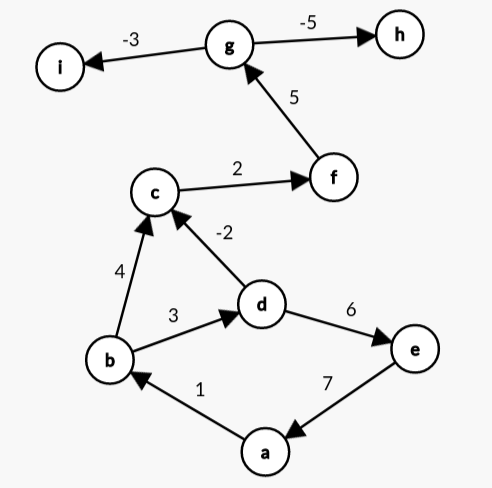
\includegraphics[width=0.8\linewidth]{figs/task-9/graph-9.png}
  \end{minipage}
  \begin{minipage}{0.5\textwidth}
    \centering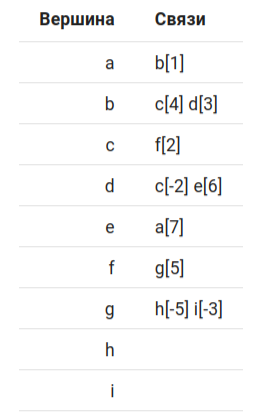
\includegraphics[width=0.6\linewidth]{figs/task-9/adj-9.png}
  \end{minipage}
  \caption{Неориентированный взвешенный граф}
\end{figure}

\begin{minted}{js}
{
  "weighted": true,
  "oriented": true,
  "adj": {
    "a": {
      "b": 1
    },
    "b": {
      "c": 4,
      "d": 3
    },
    "c": {
      "f": 2
    },
    "d": {
      "c": -2,
      "e": 6
    },
    "e": {
      "a": 7
    },
    "f": {
      "g": 5
    },
    "g": {
      "h": -5,
      "i": -3
    },
    "h": {},
    "i": {}
  }
}
\end{minted}

\subsubsection{Выходные данные}
\begin{figure}[H]
  \centering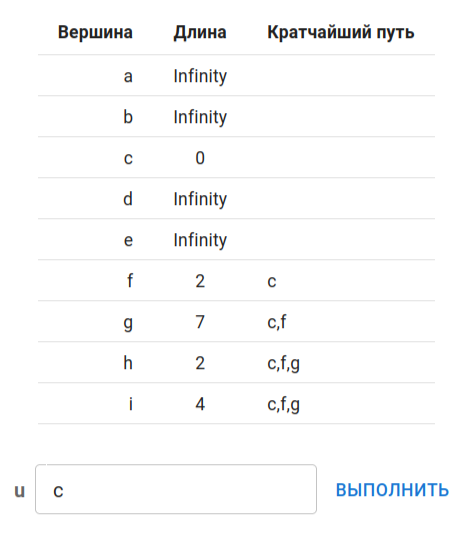
\includegraphics[width=0.6\textwidth]{figs/task-9/res-9.png}
  \caption{Результат работы}
\end{figure}